\section{Memory-augmented Online VAD}
\label{sec:theory}

\fboxsep=1mm%padding thickness
\fboxrule=1pt%border thickness

\begin{figure*}[!ht]
		%  trim={<left> <lower> <right> <upper>}
        %\fcolorbox{red}{yellow}{
            \centerline{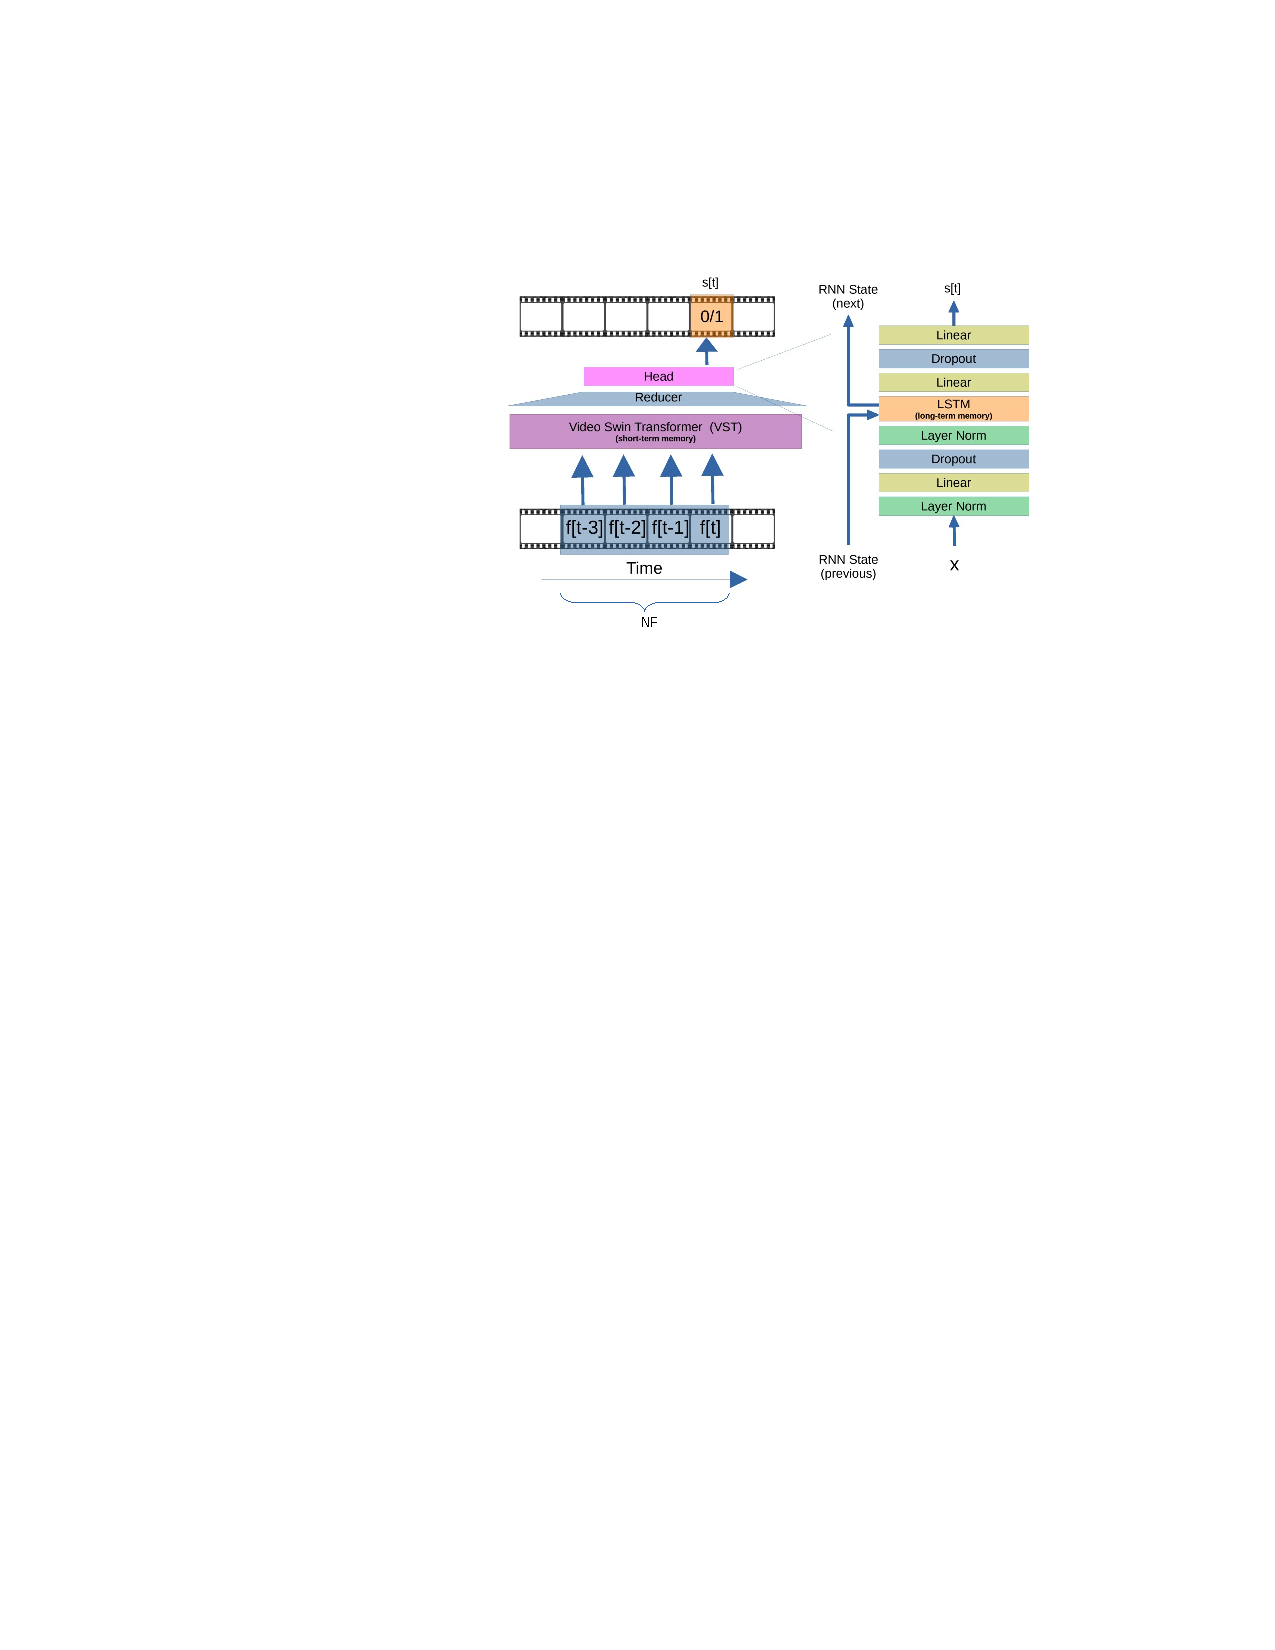
\includegraphics[trim=205 500 80 130, clip, width=0.8\linewidth]{images/arch.pdf}}
        %}
        % FIXME aggiungi link per immagine dei frame (copyright)
        \caption{The online video frame anomaly detection architecture. $f[t]$ is the frame at time $t$, $x$ the output of the Reducer.}
		\label{fig:arch}
\end{figure*}

In this section, the proposed system is described.  
The model is composed by two main blocks: a short-term memory module and a classification head that also includes a long-term  memory module (see Fig.~\ref{fig:arch}). 
The first memory module is able to keep track of both the present and the near past, while the second one will be able to also handle the remote past.
% TODO descrivere la nuova annotazione ??? Check motivazioni! :)

\noindent\textbf{Short-term memory module.}
%TODO Breve accenno su tranformer MB: SECONDO ME NON CI STA
%Taking inspiration from~\cite{xu2021long}, recently observed frames have been taken into account as a source of information related to the ongoing action, and past frames as a source of information on the context.
Since we are dealing with online anomaly frame classification, the only information available to the system, at any given time, are the current and the past frames.
In the case of the short-term memory module, only a small portion of these frames are used as input.
%Experiments will report an ablation study to justify this specific choice.\lnote{check, perchè 4 sembra meglio!}
%The network has to take the time into consideration, as incorrect behavior is often recognizable by taking into consideration the immediate past.
In order to deploy this module, we selected a Vision Transformer~\cite{DBLP:conf/iclr/DosovitskiyB0WZ21}, which has become very popular in computer vision tasks, challenging the predominance of CNN architectures. 
In particular, the Video Swin Transformer (VST)~\cite{liu_video_2022} was chosen due to its superior performance compared to a vanilla ViT~\cite{DBLP:conf/iclr/DosovitskiyB0WZ21} model
and over an RNN \tnote{such as qualcosa e poi una citazione?} given the ability to process frames in parallel.
%The VST model is the extension to video of the Swin Transformer~\cite{liu2021Swin}, which is a general-purpose image backbone with high performance on tasks that involve detection and localization.
Originally born to carry out the task of video action classification, analyzing all the frames in one step, in this work it has been adapted to perform single frame classification.
In particular, it considers only a small temporal window of $T$ frames of the video going from the current frame at time $t$ to the previous frames at time $t-T-1$.
As shown in Fig.~\ref{fig:arch}, in our case $T=3$, i.e., the input of the VST is formed by $f[t]$, $f[t-1]$ and $f[t-2]$ \tnote{io preferisco la notazione $f_t$}, where $f[y]$ represents the frame at time $y$.

VST takes as input a video with size $T \times H \times W \times 3$, where $T$, $H$ e $W$ correspond to the number of frames, height, width and RGB channels, respectively.
The model internally splits the frames in non-overlapping 3D patches, partitioning the video in $\frac{T}{2} \times \frac{H}{4} \times \frac{W}{4}$ 3D tokens, projecting the features to an arbitrary dimension $C$.
The rest of the architecture is similar to the original Swin Transformer, with four stages of Video Swin Transformer blocks, 
interspersed with $2\times$ spatial downsampling in the patch merging layer.

\noindent\textbf{Classification Head.}
The Classification Head, which generates the final output, is attached to the output of the VST after an Adaptive Average Pool 3D layer (called Reducer).
As shown in Fig.~\ref{fig:arch}, the head is composed by a series of normalization layers, linear layers and dropout, alternating. 
In addition, the Classification Head also deals with long-term memory thanks to a LSTM module inserted after the last normalization layer.





%train  dataset:  3191  video annotations found
%Normal frames found:  221429
%Anomaly frames found: 108121
%val  dataset:  1376  video annotations found
%Normal frames found:  94347
%Anomaly frames found: 46971

\noindent\textbf{Long-term memory module.}
In order to not lose information from the distant past, we need a way to keep track of it.
For this reason, we introduce a long-term memory module  which is updated whenever a new set of frames is analyzed by the system.
Specifically, we choose to employ an RNN module (LSTM \cite{lstm,gru} in this specific case).
Given that the input of the LSTM  are only the latent features, the module is very efficient and leads to a limited additional computational cost.
Indeed, it condenses all its knowledge into two states: an hidden state $h_t$ and cell state $c_t$.
Since the output of the first Linear layer of the classifier head provides the summary about the $T$ frames processed by the short-term memory model, the LSTM cells is added after it.

% copyright image frame: <a href="https://www.freepik.com/free-vector/realistic-vector-icon-film-tape-strip-with-white-square-isolated-white-cinema-concept_31096470.htm#query=video%20frame&position=31&from_view=keyword">Image by user15245033</a> on Freepik



%\noindent\textbf{Training the system.}

During the training phase, for each frame at time $t$, the model outputs the anomaly classification score $s_t \in [0,1]$, where $s_t=0$ means absence of anomaly and $s_t=1$ means the frame is surely anomalous.
A weighted cross-entropy loss was chosen, giving more weight to the anomaly class, because it is spotted less frequently \tnote{scriviamo il rapporto fra le due classi: 70/30?} \vnote{TODO: contare il numero effettivo di frame anomali/normali}.